% $Id: methodology.tex 142 2012-12-22 10:41:32Z danbos $
\chapter{Implementation proximity-based authentication scheme}
\label{ch:implementationAuth}
This chapter describes the implementation and delineates the conducted work for the design of an authentication scheme based on context.

To be able to sense the ambient data, 
in Figure \ref{fig_device} is shown how the sensors used to collect the data are connected to the \acs{RPi}. 
\begin{figure}[!h]
\centering
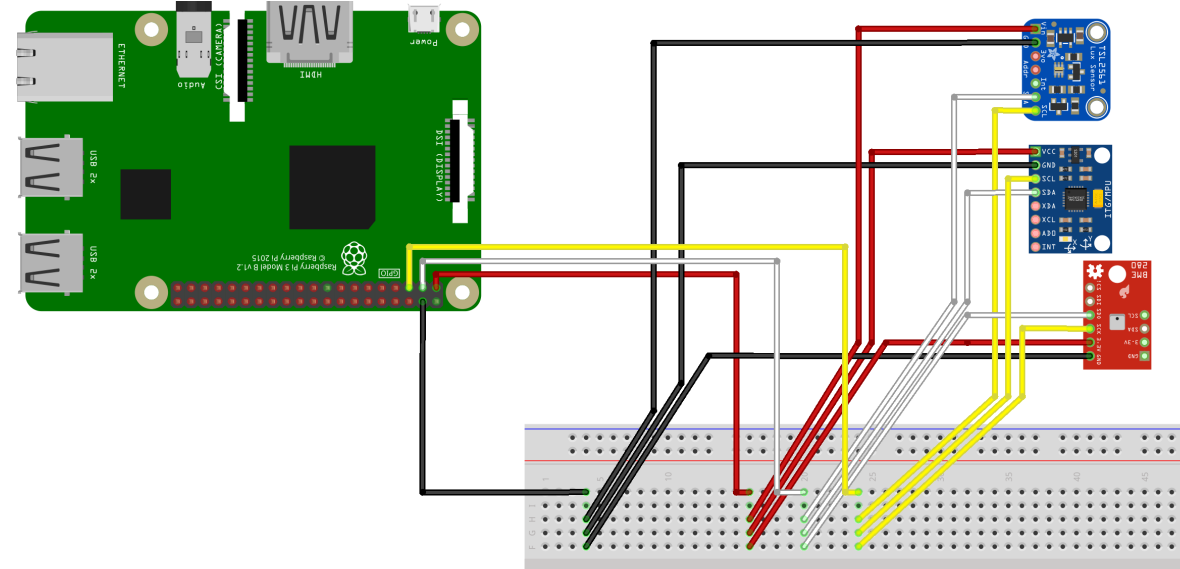
\includegraphics[width=6in]{images/device.png}
\caption{Raspberry Pi with the used context sensors.}
\label{fig_device}
\end{figure}

The  sensors direct digital output that can be sensed by the GPIO pins of the Raspberry Pi while the microphone is connected to the micro-controller through a USB sound card.
The system is using Raspbian as operating system which  is  the  massively  popular  OS for Raspberry Pi.
To get the data from the sensors have been used the following libraries:
\begin{itemize}
    \item{adafruit-circuitpython-bme280:} I2C and SPI driver for the Bosch BME280;
    \item{Adafruit\_CircuitPython\_TSL2591:} drivers for the sensors Adafruit TSL2591;
    \item{mpu6050-raspberrypi:} module for the sensor MPU6050;
\end{itemize}
The modules are all implemented in \textit{Python 3} which make easy to interact with them and to get the data.
To record audio has been used a script using the software \textit{ffmpeg} which allows the recording of audio through the sound card and its conversion to the \textit{.mp3} format in order to reduce their size.
The amount of RAM and computational power of the Raspberry  makes it commendable choice to get the real time data processed and accessed faster than other micro controller based systems.

The data sensing and the audio recording are started at the same time by a script and they save the data in file.
The tests have been executed for 24 hours, where has been constantly recorded the ambient audio and saved every 10 seconds the other ambient data.
To synchronize the start of the recording between the devices, a router has been used in order to connect them using wireless connection. 
From an external device has been sent a broadcast message to the devices connected and this triggers the start of the recording.

\section{Authentication protocol}
The authentication protocol has been implemented in $Python$ and is divided in two parts: fingerprint generation and fuzzy commitment scheme.

\subsection{Fingerprint}
The fingerprint extraction from the sensors function takes  the raw sensors data of length \textit{l\_sensor} values for each sensor and encode the signal to a fingerprint \textit{F} of length \textit{l\_F} bits. 
Two different fingerprint functions are implemented: one for the sensors and one for the audio.
\subsubsection{Fingerprint from sensor data}
The algorithm captures abrupt changes in the data and encodes them into high bits, mapping the remaining signal to low bits. 
The encoding algorithm is inspired from the one proposed in \cite{Nguyen2014Context-BasedDevices} and is divided in: 
\begin{itemize}
    \item \textbf{pre-processing:} apply a moving average filter to the raw data from each sensor. The raw data of a specific sensor are split in $k$ non overlapping segments of size $l\_segment$. A new vector $avg\_sensor$ is then generated by calculating the value's average of each segment.
    
    \item \textbf{generate fingerprint of each sensor:} we calculate each sensor data fingerprint as a sequence of bits $F_s$, in which each bit denotes the change of each $avg\_sensor$ value in comparison with the previous $avg\_sensor$ value. 
    The fingerprint bit corresponding to a value of $avg\_sensor$ is set to "1" if the relative change between two consecutive values of the vector $avg\_sensor$ is larger than a specified relative threshold $\Delta_r$ and if the difference between the values exceeds an absolute threshold value $\Delta_a$.
    In the other cases the bit is set to "0".
    \item \textbf{combine fingerprints:} the generated fingerprints $F_s$ are now concatenated in order to generate a unique context fingerprint \textit{F}. 
\end{itemize}

\subsubsection{Fingerprint from audio data}
The fingerprinting scheme is inspired by the one proposed in \cite{Schurmann2013SecureAudio}, where its security relies on the fact that the attacker is not sharing the context with the trusted devices.

In the proposed scheme, the devices start to record the sound for $t_s$ seconds generating an audio sequence $S$ with length $|S| = l_s = t_s \times r$, where $r$ is the sample rate.
The audio sequence is then split in $n_f$ frames  $S_1, \dots , S_n$ of length $|S_i| = d $ as shown in Figure \ref{fig_frames}.

\begin{figure}[!h]
\centering
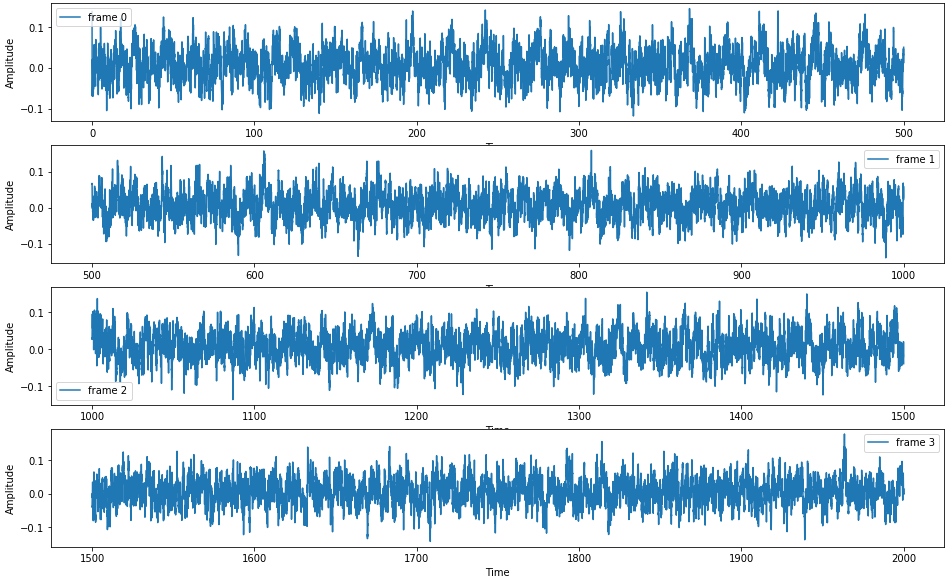
\includegraphics[width=6in]{images/frames.PNG}
\caption{Audio data split in frames. }
\label{fig_frames}
\end{figure}

On each frame is applied a discrete Fourier transformation (DTF) and calculated its absolute value (Figure \ref{fig_spectrums}):
\begin{center}
    $\forall i \in \{ 1, \dots , n \}$, 
    $FS_i = |DTF(S_i)|$
\end{center}

\begin{figure}[!h]
\centering
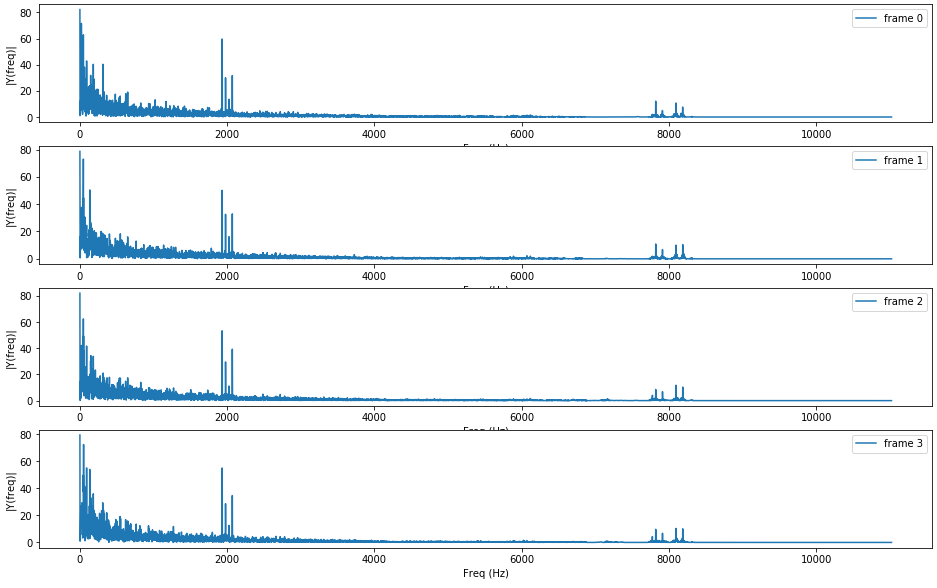
\includegraphics[width=6in]{images/spectrums.PNG}
\caption{Calculate the absolute value of the DTF on each frame. }
\label{fig_spectrums}
\end{figure}

Now the sets are summed together in order to to get a unique set of frequencies $FS_{tot}$ where the value  of the frequency $i$ is obtained by the sum of each val of $i$ of each set $S_i$.
Then a set $\overline{SF_{tot}}$ is obtained by applying an average filter of length $b$ over $FS_{tot}$ in order to remove noises as shown in Figure \ref{fig_spectrumsAVG}.

\begin{figure}[!h]
\centering
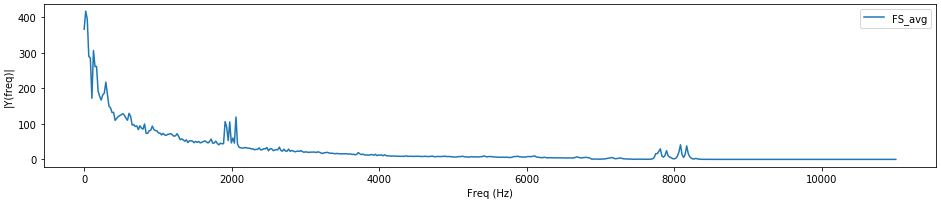
\includegraphics[width=6in]{images/spectrum_tot.PNG}
\caption{Generate $FS_{tot}$ and apply average  filter on it. }
\label{fig_spectrumsAVG}
\end{figure}

Based on the obtained sequence, it is possible to calculate the ambient audio fingerprint as a sequence of bits, in which each bit denotes the  change  of  the  $\overline{SF_{tot}}$  average value  in  comparison with  the  previous  $\overline{SF_{tot}}$'s  average.
The fingerprint bit corresponding to a value of $\overline{SF_{tot}}$ is set to "1" if the relative change between two consecutive values of the vector $\overline{SF_{tot}}$ is larger than a specified relative threshold $\Delta r_i$ and if the difference between the values exceeds an absolute threshold value $\Delta a_i$.
In the other cases the bit is set to "0".
$\Delta r$ and $\Delta a$ are two vector with the same dimension $|d_f|$ of the fingerprint and are generated by calculating the average of the relative changes  and absolute  differences between consecutive values in each frame $i \in \{0, \dots ,|d_f|-1 \}$ of $SF_{tot}$.

\subsection{Fuzzy commitment scheme}
For this part has been used the implementation proposed in \cite{fuzzyPairing}. 
This is a \textit{Python} implementation based on \cite{Juels2004AScheme} and it is divided in two main functions as shown in Figure \ref{fig_fuzzyCommit}: the commitment and the decommitment of a fuzzy commitment.
The commitment function is used to hide a randomly chosen set of bit $\kappa$ using the generated fingerprint $w$.
The decommitment method is designed in such a way that it receives a fingerprint $w'$ and if the Hamming distance is $Hamming(w , w') \leq t$ it can regenerate $\kappa$.

To implement these functions has been used a Reed-Solomon Python extension module based on the fast, GPL Reed-Solomon library by Phil Karn.
%%http://www.ka9q.net/code/fec/
The Reed-Solomon code $RS(q,m,n)$, with $q=2^k, k \in \mathbf{N} $ and $n <2^k$, is used to encode the random $\kappa$ to a codeword $c$ and to generate an "helper" value $\delta = c \oplus w$. 
During the decommitment phase, the Reed-Solomon scheme is used to decode a value $c' = w' \oplus \delta$ and get the value $\kappa$.
This procedure is capable of correcting up  to
\begin{center}
    $t = \dfrac{n - m }{2}$
\end{center}
differing  bits  between  the fingerprints.

\begin{figure}[!h]
\centering
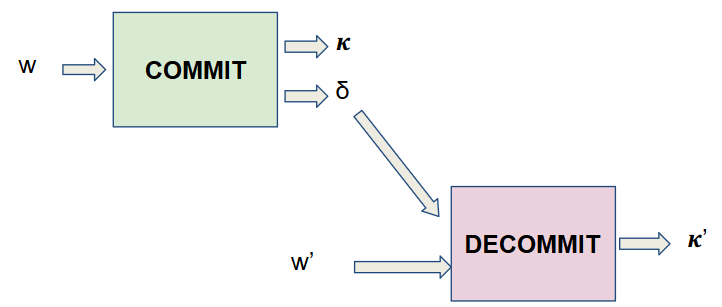
\includegraphics[width=4.5in]{images/fuzzy.PNG}
\caption{Fuzzy commitment scheme methods. }
\label{fig_fuzzyCommit}
\end{figure}